\section{Results}
\label{sec:results}

\begin{figure*}[t]
\centering
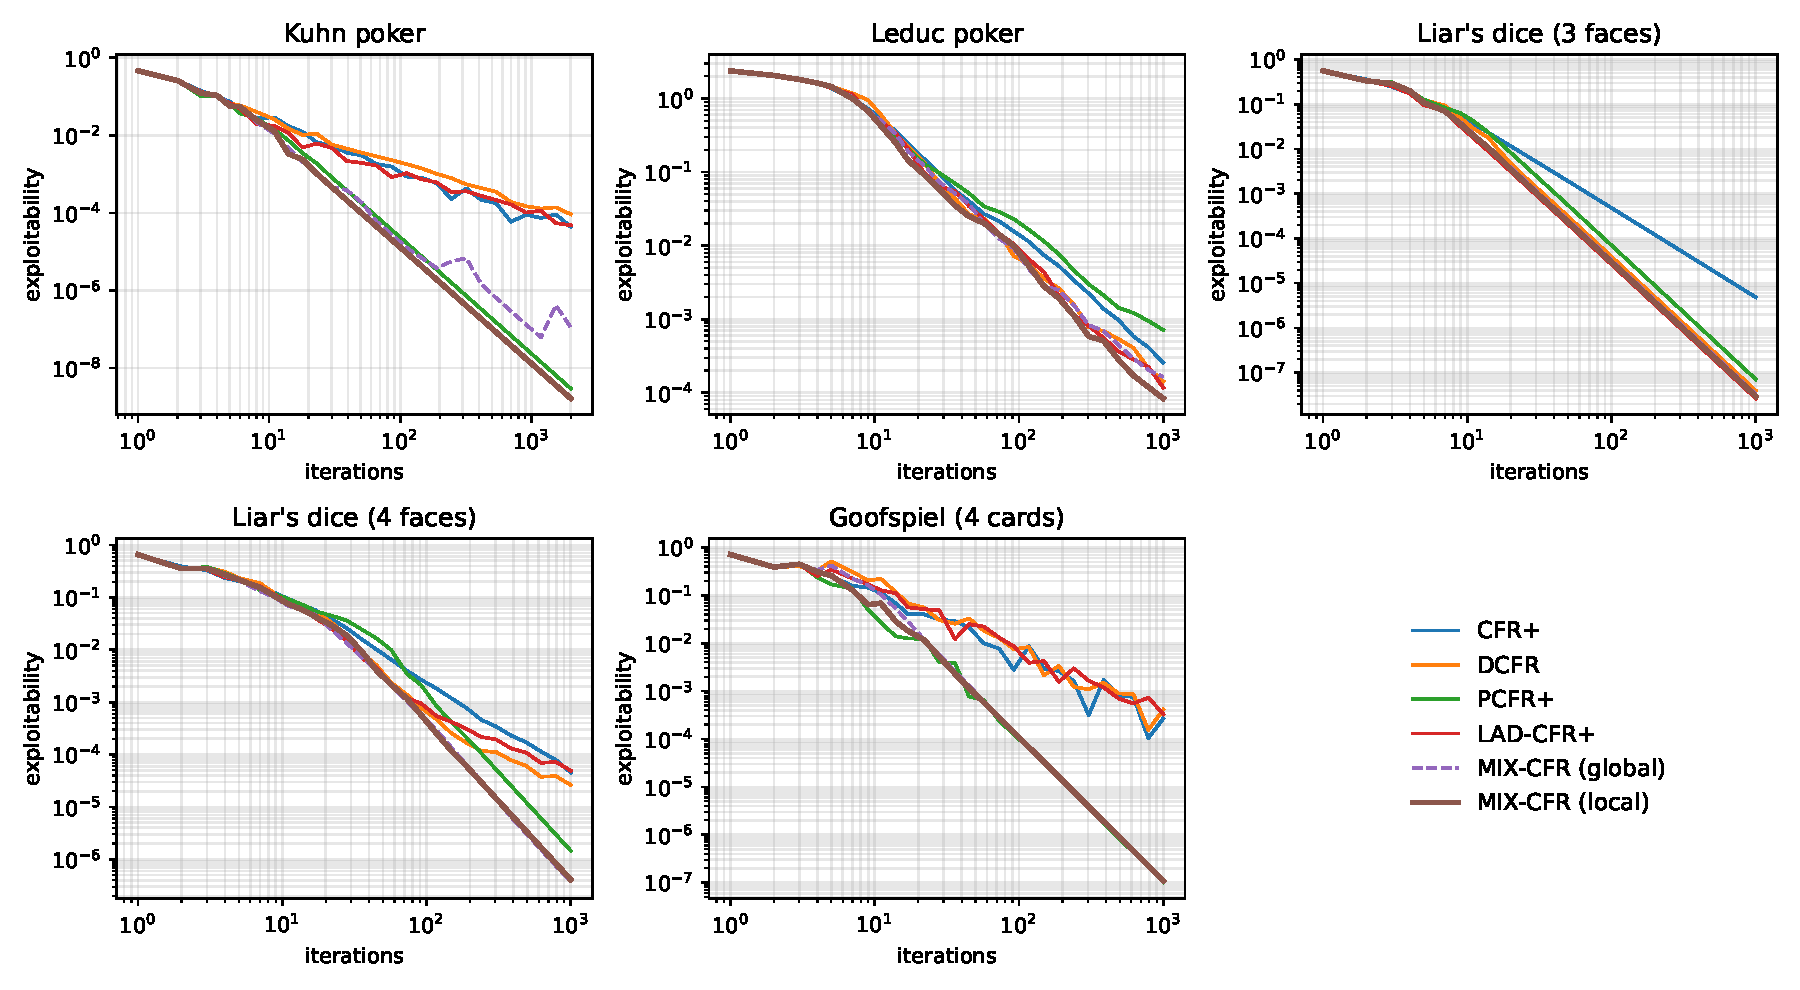
\includegraphics[width=0.92\textwidth]{figures/convergence.pdf}
\caption{Exploitability of the average strategy versus iterations (log--log). MIX-CFR
(local, thick line) is the best or close to the best method on every game, while each fixed
rule is clearly behind on at least one game.}
\label{fig:convergence}
\end{figure*}

\begin{table*}[t]
\centering
\caption{Exploitability after the final iteration (Table~\ref{tab:games}); lower is better,
best in bold. The best setting of \ours{} was selected on Kuhn and Leduc poker.}
\label{tab:main}
\begin{tabular}{@{}lcccccc@{}}
\toprule
\textbf{Game} & \textbf{\cfrp{}} & \textbf{DCFR} & \textbf{\pcfrp{}} & \textbf{\ours{}} &
\textbf{MIX-CFR (global)} & \textbf{MIX-CFR (local)} \\
\midrule
Kuhn poker           & $4.4\times10^{-5}$ & $9.2\times10^{-5}$ & $2.9\times10^{-9}$ & $4.8\times10^{-5}$ & $1.1\times10^{-7}$ & $\mathbf{1.6\times10^{-9}}$ \\
Leduc poker          & $2.6\times10^{-4}$ & $1.4\times10^{-4}$ & $7.1\times10^{-4}$ & $1.2\times10^{-4}$ & $1.6\times10^{-4}$ & $\mathbf{8.4\times10^{-5}}$ \\
Liar's dice (3)      & $4.8\times10^{-6}$ & $4.0\times10^{-8}$ & $7.1\times10^{-8}$ & $\mathbf{2.7\times10^{-8}}$ & $3.3\times10^{-8}$ & $3.0\times10^{-8}$ \\
Liar's dice (4)      & $4.5\times10^{-5}$ & $2.6\times10^{-5}$ & $1.5\times10^{-6}$ & $4.9\times10^{-5}$ & $\mathbf{3.7\times10^{-7}}$ & $4.1\times10^{-7}$ \\
Goofspiel (4)        & $2.7\times10^{-4}$ & $4.1\times10^{-4}$ & $\mathbf{1.0\times10^{-7}}$ & $3.3\times10^{-4}$ & $1.1\times10^{-7}$ & $1.1\times10^{-7}$ \\
\bottomrule
\end{tabular}
\end{table*}

\textbf{No fixed rule wins everywhere.} Table~\ref{tab:main} and Fig.~\ref{fig:convergence}
show that the ranking of the existing methods depends strongly on the game. \pcfrp{} is the
best fixed rule on Kuhn poker, Liar's dice with four faces and Goofspiel, but the worst method
on Leduc poker, where it is $2.8\times$ worse than \cfrp{}. DCFR is the best fixed rule on Leduc
poker but is worse than \cfrp{} on Kuhn poker and Goofspiel.

\textbf{MIX-CFR is consistently strong.} The local version of MIX-CFR is the best method on Kuhn
poker ($1.8\times$ lower exploitability than \pcfrp{}) and Leduc poker ($1.7\times$ lower than
DCFR, $3.1\times$ lower than \cfrp{}), and within $1.13\times$ of the best method on the other
three games. On Leduc poker and on Liar's dice with four faces, it is better than every
expert it combines: $3.6\times$ better than \pcfrp{} on the latter. It is the only method that is
not far behind the best on any game, and it achieves this without any tuning.

\textbf{Local versus global.} With the same experts, the local meta learner is $69\times$ better
than the global one on Kuhn poker and $2.0\times$ better on Leduc poker. It is slightly better on
Liar's dice with three faces, equal on Goofspiel, and $1.1\times$ worse on Liar's dice with four
faces. On Kuhn poker, the local learners give DCFR an average weight of $0.32$, compared with
$0.10$ for the global learner after 2000 iterations, which shows that information sets differ in which rule
suits them.

\textbf{Locally adaptive discounting.} Table~\ref{tab:lad} isolates the effect of the adaptive
discount. Compared with \cfrp{} using the same $t^2$ averaging, \ours{} lowers exploitability on
four of five games, including $1.8\times$ on Leduc poker. The local version is better than the
global version with the same settings on all five games. However, adapting only the discount
does not close the gap to the best fixed rule: \ours{} is worse than plain \cfrp{} on Liar's
dice with four faces and Goofspiel, and far behind \pcfrp{} on Kuhn poker and Goofspiel. Its
results were also sensitive to its settings. Discounting more strongly than DCFR at volatile
information sets increased exploitability by one to two orders of magnitude on both tuning
games.

\begin{table}[t]
\centering
\caption{Isolating the adaptive discount: exploitability of \cfrp{} variants with
$t^2$ averaging. ``Uniform'' applies the DCFR discount ($\alpha=3/2$) at every information set.}
\label{tab:lad}
\setlength{\tabcolsep}{3pt}
\begin{tabular}{@{}lcccc@{}}
\toprule
\textbf{Game} & \textbf{\cfrp{}} & \textbf{Uniform} & \textbf{\ours{} glob.} & \textbf{\ours{}} \\
\midrule
Kuhn         & $7.4\times10^{-5}$ & $4.8\times10^{-5}$ & $1.2\times10^{-4}$ & $\mathbf{4.8\times10^{-5}}$ \\
Leduc        & $2.1\times10^{-4}$ & $1.9\times10^{-4}$ & $1.4\times10^{-4}$ & $\mathbf{1.2\times10^{-4}}$ \\
Liar's d.\ (3) & $3.0\times10^{-8}$ & $3.9\times10^{-8}$ & $2.9\times10^{-8}$ & $\mathbf{2.7\times10^{-8}}$ \\
Liar's d.\ (4) & $4.5\times10^{-5}$ & $\mathbf{3.5\times10^{-5}}$ & $5.2\times10^{-5}$ & $4.9\times10^{-5}$ \\
Goofspiel    & $4.0\times10^{-4}$ & $\mathbf{1.1\times10^{-4}}$ & $5.6\times10^{-4}$ & $3.3\times10^{-4}$ \\
\bottomrule
\end{tabular}
\end{table}

\begin{table}[t]
\centering
\caption{MIX-CFR ablations: exploitability relative to the full method (values above 1 are
worse).}
\label{tab:ablation}
\setlength{\tabcolsep}{3pt}
\begin{tabular}{@{}lccccc@{}}
\toprule
\textbf{Variant} & \textbf{Kuhn} & \textbf{Leduc} & \textbf{LD(3)} & \textbf{LD(4)} & \textbf{Goof.} \\
\midrule
without \cfrp{}       & 866   & 2.20 & 1.23 & 0.90 & 24.2 \\
without DCFR          & 0.94  & 1.89 & 0.96 & 1.01 & 0.67 \\
without \pcfrp{}      & $3.7\times10^{4}$ & 1.49 & 1.01 & 30.9 & 2700 \\
predictive meta       & 1.13  & 1.41 & 1.00 & 1.05 & 29.7 \\
global meta           & 68.5  & 1.97 & 1.11 & 0.90 & 1.03 \\
\bottomrule
\end{tabular}
\end{table}

\textbf{Ablations.} Table~\ref{tab:ablation} shows that every expert matters somewhere.
Removing \pcfrp{} increases exploitability by factors of $31$ to $3.7\times10^{4}$ on Kuhn
poker, Liar's dice with four faces and Goofspiel, and removing \cfrp{} hurts on four of five games. DCFR is needed mainly on
Leduc poker, where removing it nearly doubles exploitability, which is the game where DCFR is
the best fixed rule. A predictive meta learner does not help and is $30\times$ worse on
Goofspiel, so we use plain regret matching$^+$.

\textbf{Cost.} MIX-CFR updates three experts per information set, but the tree traversal
dominates the running time. Its wall-clock time per run was between $0.9\times$ and
$1.5\times$ that of \cfrp{}. These timings were measured with eight runs in parallel on one
machine, so they are approximate.
